\section{Resultados e discussões}

\subsection{Mudança de fase} % Mudança de fase da água
Ao aquecer o recipiente com um pouco de água dentro e depois mergulhá-lo de ponta cabeça na água, foi possível observar a água preencher o volume do recipiente por inteiro. Não foi possível testar com o recipiente completamente seco pois já estava molhado pelo uso de grupos anteriores. No entanto, o esperado seria que da mesma forma a água preenchesse o volume do recipiente, porém não por inteiro. 

O princípio por trás desta diferença entre o recipiente com água ou sem água está na mudança de fase da água. Primeiro, vamos fazer a análise geral do fenômeno, depois discutiremos em termos das diferenças. 

Em ambos os casos, ao aquecer o frasco, a velocidade média das partículas nele aumenta, como o frasco é um sistema aberto, a pressão se mantém constante e igual a pressão atmosférica, o volume do frasco é fixo, então pela lei geral dos gases ideais, temos que o número de mols dentro do frasco deve diminuir para compensar o aumento da temperatura. Fisicamente, interpreta-se que parte das moléculas de gás são ejetadas do frasco de forma que as que sobram lá dentro, naquela temperatura, exercem pressão equivalente a \qty{1}{atm}. Ao pôr o frasco de ponta cabeça no recipiente com água, o gás agitado dentro do frasco passa a colidir com as moléculas de água, transferindo momento linear para estas, ou seja, há transferência de calor. Este processo faz com que a temperatura dentro do frasco e na água comece a entrar em equilíbrio, resfriando o gás dentro do frasco. Agora, a temperatura diminui, a princípio não há como entrar mais moléculas de gás, o volume do frasco continua constante, então, por consequência a pressão dentro do frasco torna-se menor que a pressão atmosférica. Com isso, a diferença de pressão dentro e fora do frasco gera uma força resultante sobre a água que aponta para dentro do frasco, fazendo a água subir.

Quanto à diferença entre o frasco com água ou seco antes de aquecer, a presença de água dentro do frasco faz com que a força resultante da diferença de pressão seja maior. A justificativa está na mudança de fase da água, ao ser aquecida, a água torna-se vapor de água, comportando-se como gás e contribuindo para o equilíbrio de pressão previamente descrito. No entanto, ao resfriar quando o frasco é colocado de ponta cabeça no recipiente o vapor condensa e deixa de atuar como gás, exercendo ainda menos pressão contra os contornos do frasco. Isto faz com que uma porção maior do frasco seja preenchida por água do que caso o frasco estivesse completamente seco antes de aquecer.

\subsection{Motor de Heron} % Mudança de fase
Ao acender a lamparina sob o reservatório de água em princípio nada aconteceu. No entanto, após alguns instantes, vapor começou a ser ejetado dos tubos e o motor ganhou movimento angular. 

O motor funciona o seguinte processo: a água dentro do reservatório é aquecida gerando vapor; o vapor se acumula aumentando a pressão interna, o vapor escapa gerando movimento. Segue desta maneira até que a água dentro do reservatório acabe.

Ao aquecer a água e aumentar a pressão interna, gera-se uma força resultante que aponta para fora do reservatório exatamente nos bicos do motor. Esta força faz com que o vapor seja expelido do reservatório. Pela conservação de momento linear do sistema e visto que o sistema parte do repouso, temos a seguinte relação para a velocidade do motor \(V\), a massa dentro total do motor com o tanto de água no reservatório \(M\), a velocidade com que o vapor é expelido \(v_e\) e a massa de vapor expelida \(m\):

\begin{align*}
    M \frac{dV}{dt}  = \frac{dm}{dt} v_e  \\
\end{align*}

Ou seja, a força sobre o motor é igual a \(v_e \frac{dm}{dt}\), como o vapor é expelido das pontas da esfera, então esta força resulta em um torque \(\tau\) descrito por:

\begin{align*}
    \tau = r \cdot v_e \frac{d m}{dt}  
\end{align*}

Em que \(r\) é o comprimento do tubo.

Embora seja um motor de construção relativamente simples, o motor de Heron apresenta dificuldade de escalonamento. Pelas relações apresentadas temos que para aumentar a potência do motor seria necessário: (1) aumentar o comprimento dos tubos, aumentando o torque; (2) aumentar a quantidade de calor fornecida,  aumentando \(v_e\) e a quantidade de massa expelida que também aumentam o torque; (3) otimizar a área transversal dos tubos para que a vazão aumente sem que esse aumento na vazão seja compensando por menor força resultante da diferença de pressão. A ideia (1) tem o problema de tornar um reservatório pequeno muito grande com relação ao comprimento do tubo. A ideia (2) é limitada pela disponibilidade de energia térmica. Por fim, a ideia (3) é limitada pela relação ideal, após atingi-la não há nada mais que possa ser feito.

\subsection{Pistão de sopro} % Como assoprar faz um pistão mover
Ao soprar com força a seringa observou-se que o sopro empurrou a ampola, e como a ampola estava ligada a ao disco por uma haste, seu movimento fez com que o disco iniciasse um movimento de rotação, e empurrasse a ampola para trás, reiniciando o ciclo do movimento, similar ao funcionamento de uma roda de trem. Assim, viu-se que ao assoprar a ampola em um ritmo correto, foi possível fazer o disco girar mais rápido e de forma homogênea como uma roda. 

Este experimento demonstra o principio da realização de trabalho por um gás, transformando a expansão do gás em rotação. Pois, ao soprar a seringa, aumenta-se a pressão do ar no seu interior, e como a pressão de um gás exerce uma força igual para todas as direções, uma parte dessa força move a ampola, que ligada ao disco, transforma a energia contida no ar em energia cinética do disco. Apesar de ser uma demonstração de um sistema de ação única e ciclo aberto, não produzindo trabalho continuo, serve para demonstrar como ocorre dentro de motores mais complexos, como o funcionamento de pistões por exemplo.

\subsection{Motor de Stirling} % Duas versões, combustão externa como vantagem
Foram observadas duas versões do motor de Stirling, um composto de uma seringa ligado a um compartimento de vidro com bolinhas de gude, e outro mais clássico com uma parte de metal, um dissipador de calor e uma roda.

Sobre o primeiro motor, observou-se que ao acender a lamparina em sua ponta, após um tempo, a seringa começou a levantar fazendo com que a parte de vidro com a bolinhas se inclinasse para próximo á fonte de calor e as bolinhas rolassem para o a extremidade inclinada, seguidamente observou-se que a seringa abaixou, fazendo assim com que as bolinhas voltassem para sua extremidade de origem e repetissem esse ciclo.
Agora, sobre o segundo motor, observou-se que após acender a lamparina em sua extremidade cilíndrica de metal não demorou muito tempo para que houvesse a movimentação de um pistão na outra extremidade que ligado a uma roda a fazia girar cada vez mais rápido, até atingir uma velocidade constante.

Apesar de possuírem construções bem diferentes, ambos motores partem do mesmo principio físico de funcionamento, movendo uma quantidade fixa de um gás entre uma fonte de calor e um dissipador. Esse processo define o ciclo de Stirling, que é um ciclo fechado e pode ser divido em quatro etapas termodinâmicas.
O princípio geral baseia-se na lei dos gases ideias \( (PV = nRT)\): quando um gás é aquecido, ele se expande; quando é resfriado ele se contrai. O motor de Stirling utiliza essa propriedade de forma cíclica para produzir um trabalho mecânico.

Para descrever o ciclo de Stirling fisicamente, tomaremos como exemplo o segundo motor observado, cuja construção é do tipo beta. Este motor possui uma câmara selada com uma fonte de calor em uma extremidade e um dissipador de calor na outra. No seu interior operam dois pistões: o pistão deslocador, responsável por mover o gás entre as zonas quente e fria, e o pistão de potência, que realiza o trabalho mecânico e está conectado ao volante (a roda). O ciclo do motor de Stirling ocorre em quatro etapas coordenadas, como demonstrado na \cref{MotorStirling}:

\begin{figure}[H]
	\centering
	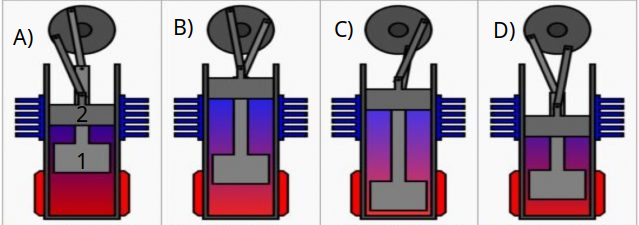
\includegraphics[width=0.80\linewidth]{fig/StirlingGenerico.png}
	\caption{A imagem ilustra as etapas sequenciais (A-D) do funcionamento do motor. O componente interno (1) é o pistão deslocador, responsável por mover o gás entre a fonte de calor (região vermelha) e o dissipador (região azul). O componente externo (2) é o pistão de potência, que realiza o trabalho mecânico acionando o volante (roda). Fonte: Adaptado de Galante et al.\cite{galante_2017}.}
	\label{MotorStirling}
\end{figure}

Primeiro, o pistão deslocador move a massa de gás para a extremidade quente da câmara (D). O gás absorve calor, e sua pressão aumenta consideravelmente. Em seguida, essa alta pressão impulsiona o pistão de potência, que se expande e realiza trabalho, transferindo energia para o volante (A).

Com o movimento contínuo do sistema, o pistão deslocador então move o gás aquecido da extremidade quente para a fria (B). O gás cede calor ao dissipador, e sua pressão diminui drasticamente (C). Finalmente, impulsionado pela inércia do volante, o pistão de potência comprime o gás frio de baixa pressão (D), deslocando a massa de gás para a extremidade quente da câmara. O ciclo então se repete, produzindo trabalho líquido a cada volta do volante.
 
Além da análise mecânica, o funcionamento do motor pode ser compreendido do ponto de vista termodinâmico, sendo o diagrama Pressão vs. Volume (P-V) a ferramenta ideal para isso, como ilustrado na \cref{CicloStirling}. Este gráfico representa as transformações que o gás de trabalho, um sistema fechado, sofre a cada etapa do ciclo.

\begin{figure}[H]
	\centering
	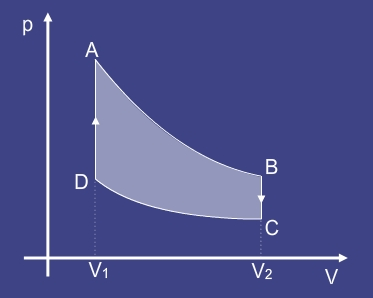
\includegraphics[width=0.30\linewidth]{fig/CicloStirling.png}
	\caption{Diagrama Pressão vs Volume do ciclo de Stirling, em que o gráfico ilustra as quatro transformações termodinâmicas do ciclo: \(D \rightarrow A\) (aquecimento isocórico), \(A \rightarrow B\) (expansão isotérmica), \(B \rightarrow C\) (resfriamento isocórico) e \(C \rightarrow D\) (compressão isotérmica). Fonte: \cite{CicloDeStirling}.}
	\label{CicloStirling}
\end{figure}

O ciclo inicia com o processo de aquecimento a volume constante (isocórico), \(D \rightarrow A\) no gráfico. Nesta fase, o gás é movido para a fonte quente e, sem que seu volume mude, sua temperatura e pressão aumentam consideravelmente. Em seguida, ocorre a expansão a temperatura constante (isotérmica), mostrada no processo \(A \rightarrow B\). Mantendo-se em contato com a fonte quente, o gás se expande, empurrando o pistão de potência para realizar trabalho. Durante esta expansão, o sistema absorve calor para manter a temperatura estável, enquanto seu volume aumenta e a pressão diminui. Esta é a fase de potência do motor.

Após a expansão, o ciclo prossegue com o resfriamento a volume constante (isocórico), no processo \(B \rightarrow C\). O gás é então deslocado para a fonte fria, onde sua temperatura e pressão caem drasticamente, mas seu volume é mantido fixo. Finalmente, a quarta etapa é a compressão a temperatura constante (isotérmica), no processo \(C \rightarrow D\). O gás é comprimido de volta ao seu volume inicial enquanto permanece em contato com a fonte fria, liberando o calor gerado no processo e fechando o ciclo, que se repetirá.

A análise a partir do gráfico P-V do ciclo de Stirling se mostra muito importante, visto que a partir da integral desse gráfico é possível obter-se o trabalho realizado pelo gás, e consequentemente a energia que é transmitida para a roda e se torna energia cinética.

O motor de Stirling possui vantagens objetivas sobre os motores convencionais, uma de suas principais vantagens é a utilização de uma combustão externa, o que possibilita a utilização de qualquer fonte de calor para o seu funcionamento, o que pode torna-lo muito mais ecológico, com a utilização de fontes de calor como energia solar concentrada, e seguro por não depender de explosões internas. Porém, os motores de Stirling possuem problemas para mudanças de potência, dependendo da intensidade das fontes de calor e de frio para realizar essas mudanças. 

\subsection{Máquina térmica} % Simplesmente concatenação de um motor com geração de energia elétrica, seque acho que tenhamos que discutir, mas é bom pelo menos citar
No experimento com a máquina térmica, observou-se que ao acender a lamparina sob o tambor de ferro - semelhante ao sistema de locomotivas - a roda externa começou a girar rapidamente. Através de um sistema de corda conectando a roda a um gerador, foi possível acender um LED, comprovando a geração de corrente elétrica a partir a energia cinética realizada pelo motor.

O funcionamento das locomotivas a vapor, como a representada no experimento, baseia-se na conversão de energia térmica em mecânica através de um ciclo termodinâmico de quatro etapas. Inicialmente, a água é aquecida na caldeira por combustão externa, gerando vapor em alta pressão e temperatura, que é então conduzido ao cilindro principal.

Na fase de expansão, o vapor pressurizado movimenta o pistão, convertendo energia térmica em trabalho mecânico. O movimento linear do pistão é transformado em rotação através de um sistema que inclui um volante de inércia. A etapa final consiste na exaustão, quando o vapor já expandido é liberado para a atmosfera ou direcionado a um condensador em sistemas fechados.

Entre as principais vantagens desses motores destacam-se a versatilidade de combustíveis (devido à combustão externa, permitindo uso de carvão, biomassa ou energia solar) e o alto torque inicial, ideal para aplicações pesadas. Essas características foram fundamentais durante a Revolução Industrial. Contudo, fatores como dimensões excessivas, longo tempo de aquecimento, riscos operacionais e significativo impacto ambiental (com emissões de poluentes) limitam sua aplicação atual.
